\section{Implementation}
The hardware description of the implemented game pong is divided into six modules. Firstly the video controller, which implements the VGA respectively HDMI interface, provides the functionality to display the video output on a monitor. Two modules generate the inputs for the movement of the paddles. The right paddle is controlled by the debounced up and down buttons of the board and the right paddle is controlled by the computer opponent. Additionally the image generator creates all required objects like the ball and paddles as well as their movement. Furthermore the match controller manages the interactions between the objects and the state of the match itself. Lastly the audio output is created by the sound generator module.
	\subsection{Video Controller}
    The video controller provides an interface for the image generator so objects can easily be displayed on a monitor. Thereby it makes the coordinates of the current pixel available and hides all additional requirements of the protocol like timing. The point of origin of the pixel matrix is located at the top left corner of the monitor. Because our group has access to the Atlys Spartan-6 board with HDMI connector as well as the Nexys4 board with VGA connector, we decided to implement a video controller for both protocols, so the remaining modules could be implemented using both boards. The main focus was laid on the above mentioned uniform interface for the image generator so the remaining development is independent of the used video controller.
        \subsubsection{VGA Controller}
            The Nexys4 board contains a VGA interface with 4-bits-per-color as well as the sync signals (horizontal sync - HS, vertical sync - VS). As shown in figure~\ref{vga_inf} the analog color signal for each of the 3 colors red, green and blue is generated by resistor-divider circuits. This results in 16 signal levels per color. 
	        \begin{figure}[h]
		        \centering
		        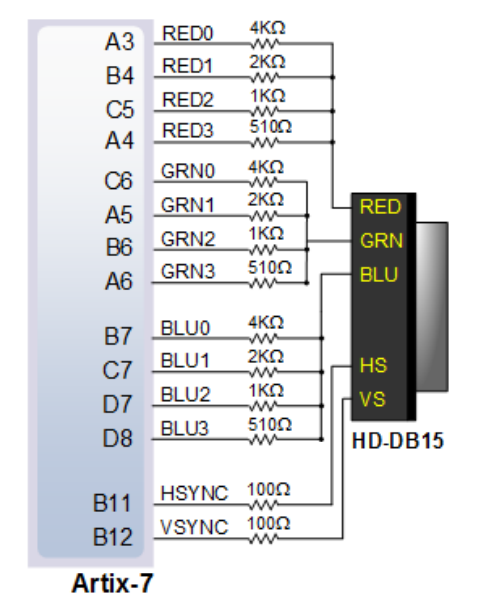
\includegraphics[scale=0.4]{images/vga_interface.png}
		        \caption{Nexys 4 VGA Interface}
		        \label{vga_inf}
	        \end{figure}
            Horizontal sync is used to get the timing for each row of the display and vertical sync for the timing for each frame. For a display resolution of 640x480 pixels a 25~MHz pixel clock is required for a vertical refresh rate of 60~Hz. Thereby the pixel clock is generated via a clock divider from the 100~MHz system clock. The required timings for both sync signals is shown in figure~\ref{vga_timing}. Through sync pulse and pulse width the waveforms of the sync signals are specified. In addition display time as well as front and back porch are needed to identify the pixel coordinates on the display. Both porch timings are historically required, because CRT-based VGA displays used electron beams to display information on a phosphor-coated screen. Thereby the beam required these porch timings to get from the end of a row to the beginning of the next row for horizontal sync as well as from the end of a frame to the beginning of the next frame for vertical sync. Modern displays also use the same timings as CRT-displays for VGA.\\
	        \begin{figure}[h]
		        \centering
		        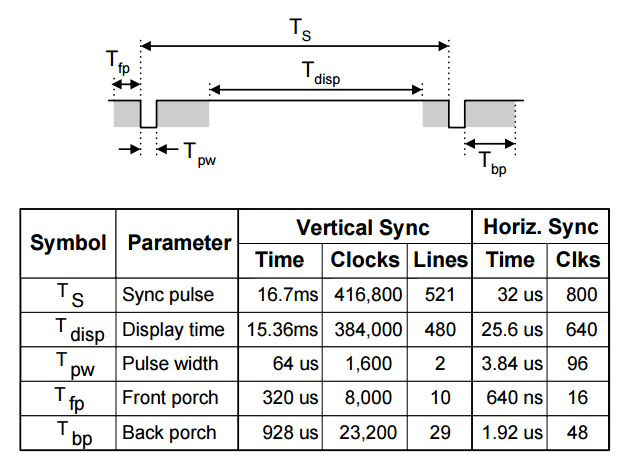
\includegraphics[scale=0.4]{images/vga_timing.png}
		        \caption{Signal timing for 640 x 480 pixels using a 25 MHz pixel clock at 60 Hz vertical refresh}
		        \label{vga_timing}
	        \end{figure}
            The VGA controller module uses two counters to generate both of these sync signals (figure~\ref{vga_sch}). In addition the display coordinates are provided for the image generator module to display all required objects.
	        \begin{figure}[h]
		        \centering
		        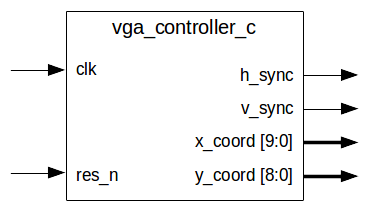
\includegraphics[scale=0.7]{images/vga_schematic.png}
		        \caption{Schematic of the VGA Controller Module}
		        \label{vga_sch}
	        \end{figure}

        \subsubsection{HDMI Controller}
    \subsection{Computer Opponent}
        Only the right paddle of the pong game is controlled by the player. So the left paddle has to be controlled by some logic. For this purpose the computer opponent module generates the button signals to move the paddle up or down. It uses the vertical position of the paddle and the ball to determine the movement of the paddle (figure~\ref{comp_sch}). A linear-feedback shift register (LFSR) is used to get some randomness into this control, so the computer opponent does not behave deterministically.
	    \begin{figure}[h]
		    \centering
		    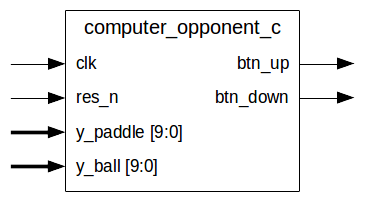
\includegraphics[scale=0.7]{images/computer_opponent_schematic.png}
		    \caption{Schematic of the Computer Opponent Module}
		    \label{comp_sch}
	    \end{figure}
    \subsection{Image Generator}
        The Image Generator takes inputs from the players (\texttt{btn\_up\_left}, \texttt{btn\_down\_left}, \texttt{btn\_up\_right}, \texttt{btn\_down\_right}) and returns the RGB values that can be displayed through the HDMI or VGA interface of the boards (figure~\ref{img_gen_sch}). The display coordinates are used in its subcomponents to show all objects at the right positions on the screen. Thereby each object is created by an individual module. Additionally four signals are received from the match controller module to ensure the right behaver of the game. The first two are \texttt{l\_scored} and \texttt{r\_scored}. These are asserted if the left respectively right player obtains a point and the movement of the ball should be reset. The other signals are \texttt{l\_paddle\_hit} and \texttt{r\_paddle\_hit}, which are asserted if the ball hits the proper paddle. The match controller receives information about the vertical position of the paddles and the position of the ball from the image generator module to generate these four signals.\\
All vectors in the schematics of the image generator and its subcomponents are matching for the resolution of the HDMI controller with 1280x720 pixels using 24-bits-colors. The schematics for the VGA resolution are not shown separately, bacause their vectors are only slightly smaller and do not change the overall structure of the modules.
	    \begin{figure}[h]
		    \centering
		    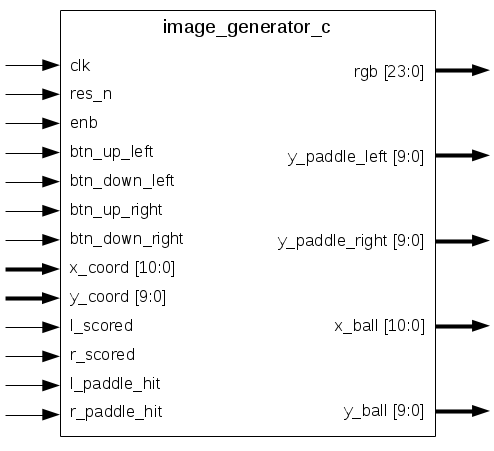
\includegraphics[scale=0.7]{images/image_generator_schematic.png}
		    \caption{Schematic of the Image Generator Module}
		    \label{img_gen_sch}
	    \end{figure}
        \subsubsection{Multiplexer}
            Because the RGB values are generated for each object individual, they have to be combined into a single output to drive the VGA connector. For this purpose a multiplexer is used (figure~\ref{mux_sch}). It forwards the RGB value of the object, which asserts its select signal. If no select is asserted, the background color is displayed. Multiple asserted select signals are resolved by using different priorities for the objects.
	        \begin{figure}[h]
		        \centering
		        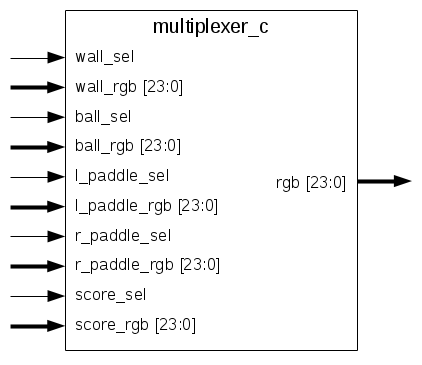
\includegraphics[scale=0.7]{images/multiplexer_schematic.png}
		        \caption{Schematic of the Multiplexer Module}
		        \label{mux_sch}
	        \end{figure}
        \subsubsection{Wall}
            To restrict the movement of the ball and the paddles the wall builds the surrounding of the field. On the basis of the display coordinates this module asserts its select signal, if the coordinates are inside of the area of the wall (figure~\ref{wall_sch}).
	        \begin{figure}[h]
		        \centering
		        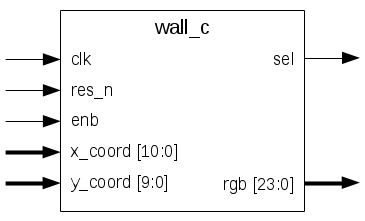
\includegraphics[scale=0.7]{images/wall_schematic.png}
		        \caption{Schematic of the Wall Module}
		        \label{wall_sch}
	        \end{figure}
        \subsubsection{Ball}
            The ball entity moving across the field is created in the \texttt{ball\_c} module (figure~\ref{ball_sch}). It moves diagonally over the field and rebound from the walls. It also rebound from a paddle, of it hits it. To indicate this, the match controller asserts \texttt{l\_paddle\_hit} or \texttt{r\_paddle\_hit}. Like the wall module, the ball module asserts its select signal, if the display coordinates are inside of the area of the ball. Additionally the coordinates of the ball (top left corner) are provided to the match controller and computer opponent modules. The right movement speed is generated by dividing the system clock down to the desired movement frequency of the ball. It then moves one pixel in x- and y-direction per movement clock cycle.
	        \begin{figure}[h]
		        \centering
		        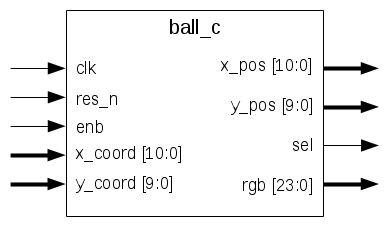
\includegraphics[scale=0.7]{images/ball_schematic.png}
		        \caption{Schematic of the Ball Module}
		        \label{ball_sch}
	        \end{figure}
        \subsubsection{Paddle}
            For each player the paddle module is instantiated. It can be moved up and down via the up- and down-buttons of the board for the right player. The values for \texttt{btn\_up} and \texttt{btn\_down} for the left player are generated by the computer opponent module. Again the display coordinates are used to assert the select signal, if the coordinates are inside of the area of the paddle (figure~\ref{paddle_sch}). Furthermore the y-position is provided to the match controller to ensure the right behaver of the match. Additionally the computer opponent receives this signal from the left paddle to calculate its movement.
	        \begin{figure}[h]
		        \centering
		        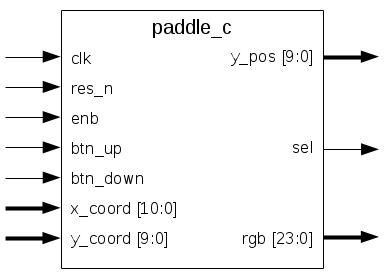
\includegraphics[scale=0.7]{images/paddle_schematic.png}
		        \caption{Schematic of the Paddle Module}
		        \label{paddle_sch}
	        \end{figure}
        \subsubsection{Score}
            A score is used to count the points each player achieves. Thereby a digit is displayed like a seven-segment display and each player can score up to 99 points (figure~\ref{score_sch}). Again the display coordinates are used to assert the select signal, if the coordinates are inside of the area of the score. Internally the score for each player is stored as a bit-vector. So it is firstly converted into BCD code and then this BCD code is used in an decoder to drive the digits of the seven-segment display.
\begin{figure}[h]
		\begin{subfigure}[b]{.5\textwidth}
            \centering
			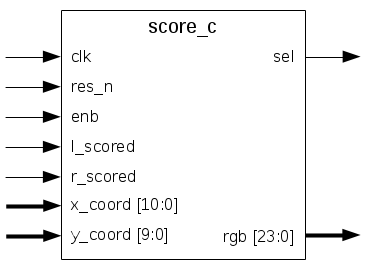
\includegraphics[scale=0.7]{images/score_schematic.png}
			\caption{Schematic of the Score Module}
		\end{subfigure}
		\hfill
		\begin{subfigure}[b]{.5\textwidth}
            \centering
			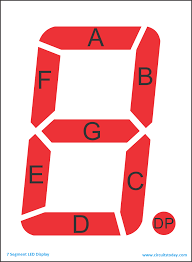
\includegraphics[scale=0.5]{images/seven_segment_display.png}		
			\caption{Seven-Segment Display}
		\end{subfigure}
        \caption{Schematic of the Score Module and Seven-Segment Display}
	    \label{score_sch}
	\end{figure}
		

    \subsection{Match Controller}
    
    \newpage
	  \subsection{Sound Generator}
				In order to generate sound, we used the on board LM4550 chip. Figure \ref{snd_gen} shows the block diagram of the sound generator. This module takes in the sound events from the Match Controller module (i.e when sound generation should take place), reads a sound effect from a ROM and sends it to the LM4550 chip that in turn outputs the sound effect to a connected speaker.
				
				The inputs to the \texttt{snd\_gen\_c} include a \texttt{clk}, an active low reset, a serial data in line \texttt{sdata\_in}, a 12.288 MHz bit clock from the AC97 chip, 3 bit \texttt{snd\_eff} signal and 5 bit \texttt{volume} control (will be connected to the switches of the Atlys board).
				
				The module's output include a \texttt{sync} signal, serial data output \texttt{sdata\_out} and an AC97 active low reset that initializes the AC97 (LM4550) chip. 
				
				Internally, the \texttt{snd\_gen\_c} module contains an AC97 controller and an AC97CMD submodules.
				\begin{itemize}
				\item \textbf{AC97 controller:} implements the AC Link serial interface protocol. Figure \ref{LM4550_protocol} shows an AC bidirectional audio frame, whereas figure \ref{LM4550_output_frame} shows an AC output audio frame. In this project, we will be using the LM4550 chip for output only, however, the input audio frame (not shown here) has also been implemented for testing reasons. The next paragraph is a brief description of the AC link interface protocol. For more details about the AC97 link serial interface protocol, see \url{http://www.ti.com/lit/ds/symlink/lm4550.pdf}
				
				The AC Link Output Frame carries control and PCM data to the LM4550 control registers and stereo DAC. Output Frames are carried on the \texttt{sdata\_out} signal which is an output from the AC97 Controller and an input to the LM4550 codec. As shown in Figure \ref{LM4550_output_frame}, Output Frames are constructed from thirteen time slots: one Tag Slot followed by twelve Data Slots. Each Frame consists of 256 bits with each of the twelve Data Slots containing 20 bits. Input and Output Frames are aligned to the same SYNC transition.
					
			\begin{figure}[h]
			\centering
				\begin{subfigure}{0.6\textwidth}
					\centering
					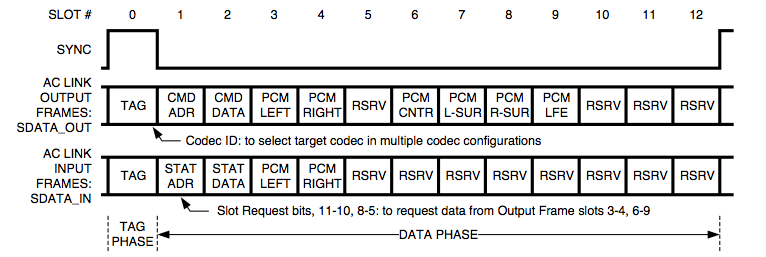
\includegraphics[scale=1]{images/LM4550_protocol.png}
					\caption{AC link bidirectional frame}
					\label{LM4550_protocol}
				\end{subfigure}
				\hfill
				\begin{subfigure}{0.6\textwidth}
					\centering
					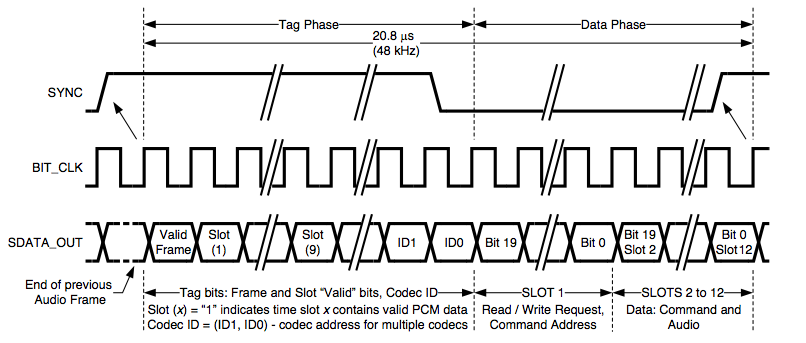
\includegraphics[scale=1]{images/LM4550_output_frame.png}
					\caption{AC link output audio frame}
					\label{LM4550_output_frame}
				\end{subfigure}
				\hfill
				\begin{subfigure}[b]{0.6\textwidth}
					\centering
					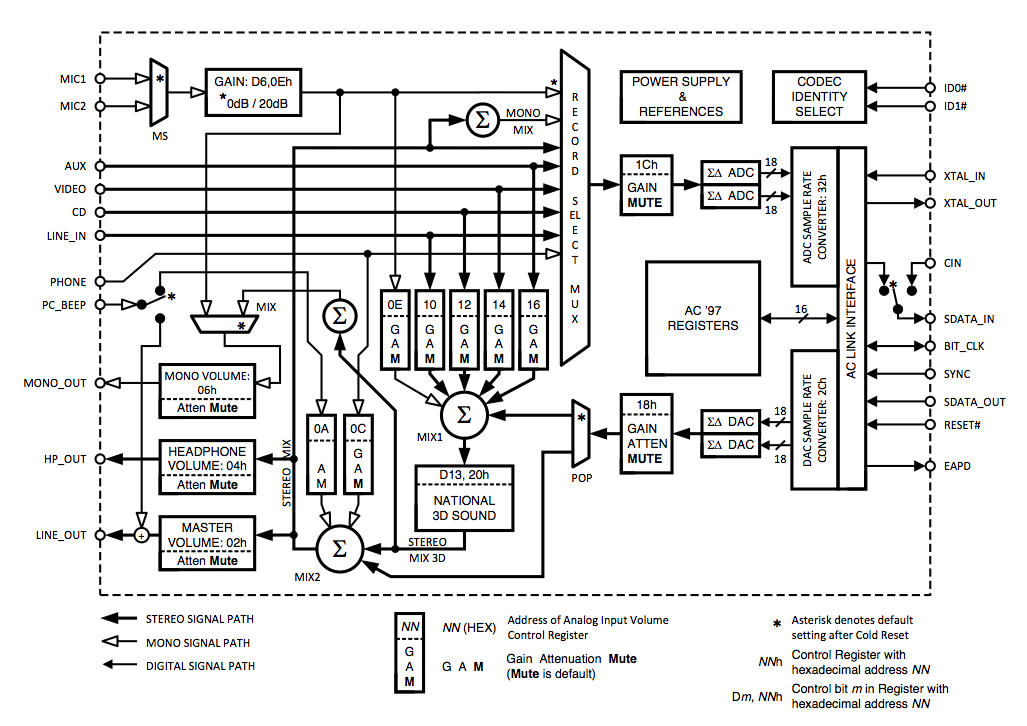
\includegraphics[scale=0.8]{images/LM4550_innen.png}
					\caption{Block diagram of LM4550 chip. Red line is the path from FPGA output to \texttt{HP\_OUT}. All registers along this path need to be configured.}
					\label{LM4550_innen}
				\end{subfigure}
				
			\caption{AC link serial interface protocol}
			\end{figure}
				\item \textbf{AC97CMD command state machine:} is a state machine that creates the control data based on the inputs \texttt{snd\_eff} and \texttt{volume} and passes it to the AC97 Controller. This control data controls among others the volume of the output audio and the DAC sample rate. Figure \ref{LM4550_innen} shows the path of the audio data that gets transferred within the LM4550 chip and the registers that need to be configured along this path. The following code was extracted from the file \texttt{a97cmd\_fsm.vhd} that implements the state machine necessary to configure the registers of the LM4550 chip. It shows an example of how to activate the output \texttt{HP\_OUT}. As shown in figure \ref{LM4550_innen} \texttt{LINE\_OUT} is muted by default. 
				
%				\begin{figure}[h]
%					\centering
%					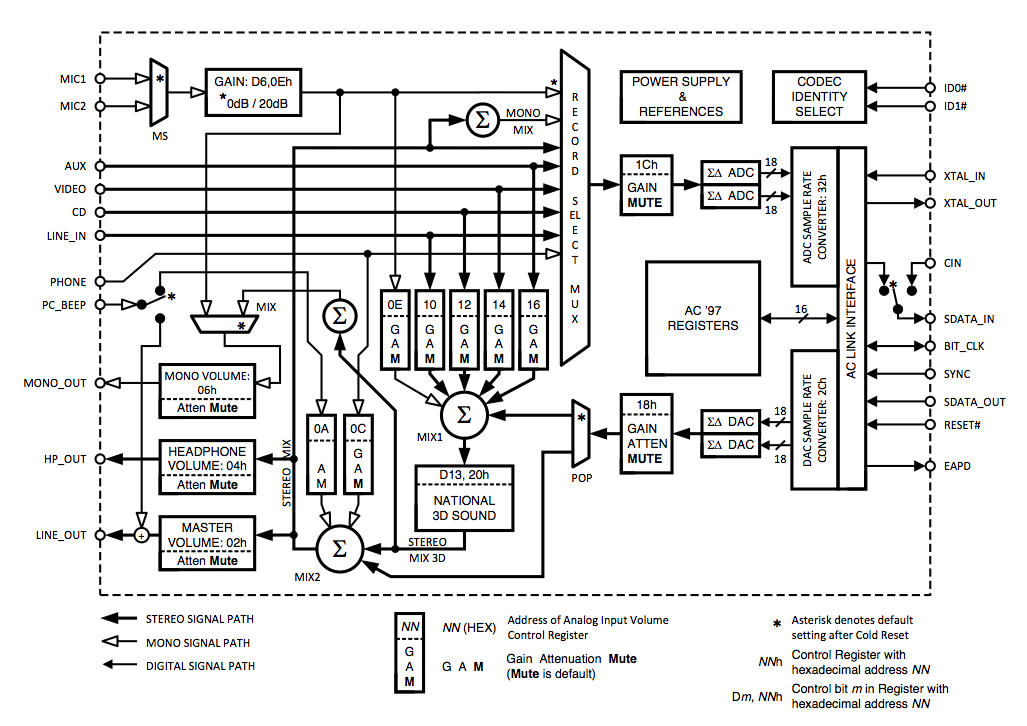
\includegraphics[scale=1]{images/LM4550_innen.png}
%					\caption{Block diagram of LM4550 chip. Red line is the path from FPGA output to \texttt{HP\_OUT}. All registers along this path need to be configured.}
%					\label{LM4550_innen}
%				\end{figure}
$\cdots$
\begin{lstlisting}
process (next_state, cur_state, atten)
    begin
        case cur_state is
    	    when S0 =>
            cmd <= X"02_8000";  -- master volume    0 0000->0dB atten, 
                                               1 1111->46.5dB atten						
                next\_state <= S2;
            when S1 => 
                                               -- HP_OUT volume
                cmd <= X"04" & "000" & atten & "000" & atten;	
                next\_state <= S4;
            when S2 => 			
		
\end{lstlisting}
$\cdots$\\
The AC97CMD module also reads the audio sound effects from a ROM that gets initialized when the FPGA is programmed. The right sound effect is chosen according to the signal \texttt{snd\_eff}.
				\end{itemize}
		  
